\section{Resultados}

\begin{table}[h]
\centering
\label{tab:results-summary}
\scriptsize
\setlength{\tabcolsep}{4pt}
\sisetup{table-format=1.3}
\begin{tabularx}{\linewidth}{@{}l X S S@{}}
\toprule
\textbf{Classifier} & \textbf{Best parameters} & {\textbf{Train acc}} & {\textbf{5-fold CV accuracy}} \\
\midrule
DecisionTree (baseline) &
\textit{defaults} &
0.670 & 0.659 \\

DecisionTree (tuned) &
\makecell[tl]{\texttt{criterion=gini, max\_depth=3,}\\
\texttt{min\_samples\_leaf=1, min\_samples\_split=2,}\\
\texttt{max\_features=None, class\_weight=None,}\\
\texttt{splitter=best}} &
0.700 & 0.719 \\

LogisticRegression &
\makecell[tl]{\texttt{C=1.0, penalty='l2', solver='lbfgs'}} &
0.732 & 0.702 \\

ExplainableBoostingMachine (GAM) &
\makecell[tl]{\texttt{learning\_rate=0.05, max\_bins=256,}\\
\texttt{interactions=5}} &
0.748 & 0.723 \\
\bottomrule
\end{tabularx}
\caption{Resumen de resultados por modelo. Los valores de \textit{Train acc} y \textit{5-fold CV accuracy} reflejan la media sobre el conjunto de entrenamiento y la validación cruzada, respectivamente.}
\end{table}

% --- Figura: matrices de confusión o comparativas por modelo ---
\begin{figure}[h]
  \centering
  \begin{subfigure}[t]{0.32\linewidth}
    \centering
    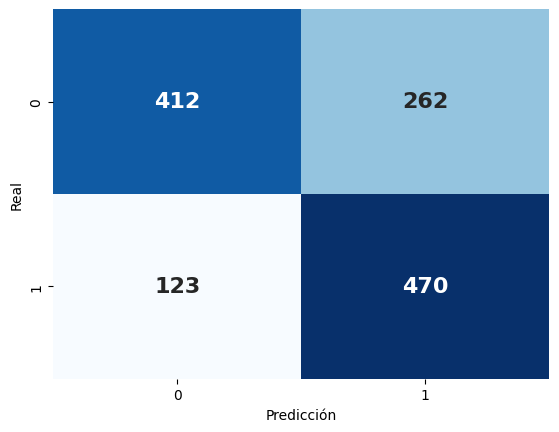
\includegraphics[width=\linewidth]{figures/decision_tree_tuned_cm.png}
    \caption{Árbol de decisión (ajustado)}
    \label{fig:cm-tree}
  \end{subfigure}\hfill
  \begin{subfigure}[t]{0.32\linewidth}
    \centering
    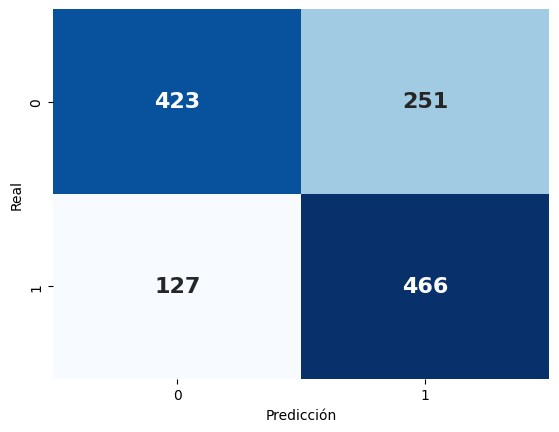
\includegraphics[width=\linewidth]{figures/logistic_cm.png}
    \caption{Regresión logística}
    \label{fig:cm-log}
  \end{subfigure}\hfill
  \begin{subfigure}[t]{0.32\linewidth}
    \centering
    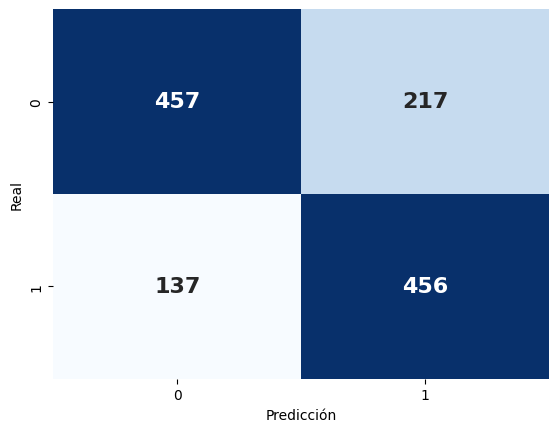
\includegraphics[width=\linewidth]{figures/ebm_cm.png}
    \caption{GAM / EBM}
    \label{fig:cm-gam}
  \end{subfigure}
  \caption{Comparativa de matrices de confusión normalizadas (0–1) para los tres modelos. El EBM presenta la mayor proporción de verdaderos positivos y falsos negativos reducidos.}
  \label{fig:cm-compare}
\end{figure}

\paragraph{Lectura breve.}
El modelo \textbf{DecisionTree (baseline)} mostró un rendimiento inicial modesto, sirviendo como referencia para validar el flujo de trabajo. 
El \textbf{DecisionTree (tuned)} logró una mejora significativa, con una \textbf{5-fold CV accuracy de 0.719}, demostrando que un árbol poco profundo y bien regularizado puede alcanzar una generalización estable.

La \textbf{Regresión Logística} ofreció un rendimiento muy equilibrado (\textbf{Train = 0.732, 5-fold = 0.702}), mostrando coeficientes coherentes con la interpretación esperada: la edad y el empleo estable reducen la probabilidad de reincidencia, mientras que el número de antecedentes la incrementa. 

Por último, el modelo \textbf{aditivo (GAM / EBM)} se consolidó como el más robusto del estudio (\textbf{Train = 0.748, 5-fold = 0.723}), manteniendo una diferencia mínima entre entrenamiento y validación. Este comportamiento indica una alta capacidad de generalización, combinando explicabilidad global (curvas de efecto) con consistencia local en las predicciones. A nivel de error, el EBM reduce falsos negativos sin aumentar excesivamente los falsos positivos, lo que lo posiciona como el modelo más equilibrado en rendimiento e interpretabilidad.
